\chapter{Implementazione}
Per realizzare la nostra estensione andremo a estendere le funzionalità di base del debugger di VSCode. I comandi di base verranno gestiti dal debugger di VSCode dopo aver configurato opportunemante il collegamento con il GDB. La nostra estensione 
si occuperà di inviare comandi per la visualizzazione dei processi attualemnte in esecuzione e mostrare i dati in una webview di VSCode.

\begin{figure}[H]
    \centering
    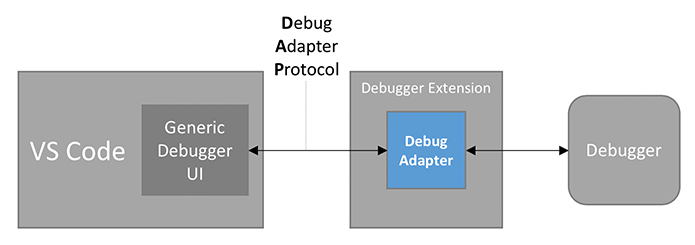
\includegraphics[width=0.7\columnwidth]{images/debug-arch2.png}
    \caption{Estensione del DP}
    \label{fig:dap dp and extension}
\end{figure}

Prima di istaurare un collegamento con il GDB vi é la necessitá di compilare ed eseguire il nucleo nella macchina QEMU. VSCode mette a disposizione il file \codeword{./vscode/task.json} all'interno della directory di lavoro. Il file permette di dichiarare dei comandi che permettono di automatizzare una moltitudine di operazioni.
\subsection*{task.json}
Il file \codeword{task.json}, come si puó evincere dall'estensione, é in formato \codeword{JSON}. I campi che lo compongono sono spiegati esaustivamente all'interno della pagina dedicata della documentazione di VSCode \cite{VSCodeTasks}. In particolare si é configurato il file per eseguire i comandi di \codeword{compile} e \codeword{boot} presenti nell'ambiente di sviluppo Linux.  

\subsubsection*{compilazione}   

\begin{figure}[H]
    \lstinputlisting[language=sh]{code/task_compile.txt}
    \caption{Compilazione}
\end{figure}

\begin{itemize}
    \item \codeword{label}: identifica univocamente il nome del task all'interno dell'ambiente
    \item \codeword{type}: come deve essere interpretato il campo \codeword{command}, in questo caso come un comando di shell
    \item \codeword{command}: il comando effettivo da eseguire
    \item \codeword{group}: definisce il gruppo a cui il task appartiene all'interno di VSCode
    \item \codeword{presentation}: sono istruzioni per VSCode su come mostrare l'output del comando all'utente 
\end{itemize}

\subsubsection*{Avvio in modalità debug}   

\begin{figure}[H]
    \lstinputlisting[language=sh]{code/task_debug.txt}
    \caption{Avvio in modalità debug}
\end{figure}

Il task di avvio in modalità debug di QEMU del nucleo richiede un campo aggiuntivo per segnalare a VSCode la terminazione del task. QEMU viene avviato in modalità debug e resta in attesa fina alla connessione del GDB. Il campo \codeword{problemMatcher} é configurato in modo tale da attendere che QEMU segnali l'attesa del GDB tramite la riga di output \codeword{INF Attendo collegamento da gdb} .

\section{Build e connessione al nucleo}
Il prerequisito per il funzionamento dell'estensione è il collegamento al GDB. Per configurarlo è stato creato il file di configurazione \codeword{launch.json} all'interno della cartella \codeword{./.vscode} dell'ambiente di lavoro. 

\subsection*{lauch.json}

\begin{figure}[H]
    \lstinputlisting[language=sh]{code/launch_conf.txt}
    \caption{launch.json}
\end{figure}

\begin{itemize}
    \item \codeword{name}: identifica univocamente il nome della configurazione del debugger
    \item \codeword{type}: richiede la tipoologia di debugger da utilizzare
    \item \codeword{request}: richiede di lanciare una nuova istanza del debugger
    \item \codeword{program}: indica quale eseguibile deve lanciare il debugger
    \item \codeword{cwd}: imposta il percorso di lavoro del debugger
    \item \codeword{miDebuggerPath}: è l'eseguibile del debugger da avviare
    \item \codeword{preLaunchTask}: richiede quali task eseguire prima di lanciare la connessione
    \item \codeword{setupCommands}: è la lista dei comandi da eseguire all'avvio del debugger
\end{itemize}

\subsubsection*{.gdbinitvscode}
GDB permette inoltre di caricare dei file di configurazione al cui interno sono definiti dei comandi di GDB, viene utilizzato per impostare le varie funzioni di visualizzazione, caricamento di ulteriori simboli o caricamento degli script personali. 

\begin{figure}[H]
    \lstinputlisting[language=sh]{code/gdbinit.txt}
    \caption{.gdbinitvscode}
\end{figure}

\section{nucleo\textunderscore vscode.py}

Il file \codeword{nucleo_debug.py} contiene la definizione di un nuovo comando per GDB: \codeword{process list}. Il comando é stato creato modificando la struttura dello script \codeword{nucleo.py}. 

\begin{figure}[H]
    \lstinputlisting[language=python]{code/nucleo.txt}
    \caption{nucleo.py}
\end{figure}

Il codice é stato modificato in modo tale da costruire come output un oggetto \codeword{JSON}

\begin{figure}[H]
    \lstinputlisting[language=python]{code/nucleo_vscode.txt}
    \caption{nucleo\textunderscore vscode.py}
\end{figure}

Il comando \codeword{process list} restituisce la lista di tutti i processi in esecuzione e le infomazioni relative al contesto del processo.

\section{Estensione Nucleo Debug}
Il funzionamento generale dell'estensione si basa sull'ascoltare quando VSCode avvia una sessione di debug. Una volta avviato il debug viene caricata una webview, questa viene aggiornata ad intervalli regolari lanciando i comandi personalizzati di GDB e formattando in HTML il risultato ottenuto dal debugger. 

\subsection{Creazione dell'estensione}
Dopo aver inizializzato l'ambiente di sviluppo per un estensione di VSCode grazie a \codeword{yeoman}, si procede alla configurazione al file di descrizione dell'estensione \codeword{package.json}. All'interno si possono definire vari campi tra cui:

\begin{itemize}
    \item \codeword{name}: identifica univocamente il nome dell'estensione
    \item \codeword{commands}: vettore di eventuali comandi che fornisce l'estensione 
    \item \codeword{activationEvents}: vettore di eventi da monitorare ai quali l'estensione viene caricata
\end{itemize}

in particolare \codeword{activationEvents} è stato popolato con l'evento \linebreak \codeword{onDebugResolve:cppdbg}, che permette di caricare l'estensione solo quando viene attivato il debug con tipo \codeword{cppdbg}.

\subsection{Caricamento dell'estensione}
Al momento del caricamento dell'estensione VSCode dall file principale \linebreak \codeword{extension.ts} chiama la funzione \codeword{activate()} al quale interno posizioniamo il codice di inizializzazione. 

\begin{figure}[H]
    \lstinputlisting[language=JavaScript]{code/activation.txt}
    \caption{activate()}
\end{figure}


\begin{itemize}
    \item \codeword{vscode.debug.onDidStartDebugSession}: permette di monitorare quando viene avviata una sessione di debug e chiamare una funzione che inizializza la webview contenente le informazioni del nucleo
    \item \codeword{vscode.debug.onDidTerminateDebugSession}: permette di monitorare quando viene terminata la sessione di debug e chiamare la funzione per pulire le schede aperte dall'estensione
\end{itemize}

\subsection{Richiesta del comando GDB}
All'interno del costruttore di \codeword{NucleoInfo} impostiamo un intervallo tramite \linebreak \codeword{setInterval(...)}, che si occuperà di gestire tutte le richieste dei comandi personalizzati di GDB tramite \codeword{customCommand(...)} e aggiornare la webview. 

\begin{figure}[H]
    \lstinputlisting[language=JavaScript]{code/costruttore.txt}
    \caption{NucleoInfo.constructor}
\end{figure}

\subsubsection{customCommand()}
\begin{figure}[H]
    \lstinputlisting[language=JavaScript]{code/customcommand.txt}
    \caption{NucleoInfo.customCommand()}
\end{figure}

La funzione \codeword{customCommand(...)} preleva il frame di esecuzione del nucleo da GDB e dopo aver costruito il comando da eseguire crea una richiesta al Debug Adapter tramite il metodo \codeword{.customRequest}, il quale istanzia una classe \codeword{ProtocolMessage} definita dal Debug Adapter Protocol di tipo \codeword{request} per richiedere l'esecuzione del commando da parte del GDB. 

\subsection{Webview}
Dopo aver recuperato tutte le informazioni del nucleo necessarie viene chiamato il metodo \codeword{_getHTMLForWebview()}. 

\begin{figure}[H]
    \lstinputlisting[language=JavaScript]{code/htmlconstruct.txt}
    \caption{NucleoInfo.\textunderscore getHTMLforwebview}
\end{figure}

Per costruire la pagina HTML che verrà caricata dalla webview utilizziamo la libreria di templating \codeword{handlebars}. Prima di poter utilizzare i dati, essi devono essere convertiti in una stuttura JSON e creato il codice HTML per la visualizzione, utilizziamo la funzione creata appositamente \codeword{formatProcessList()}, non riportata per la sua lunghezza ma disponibile nella repository del progetto \cite{formatProcessList}. 

Il codice HTML generato viene assegnato alla webview che si preoccupa di renderizzare la pagina ottenendo il seguente risultato
 
\begin{figure}[H]    
    \centering
    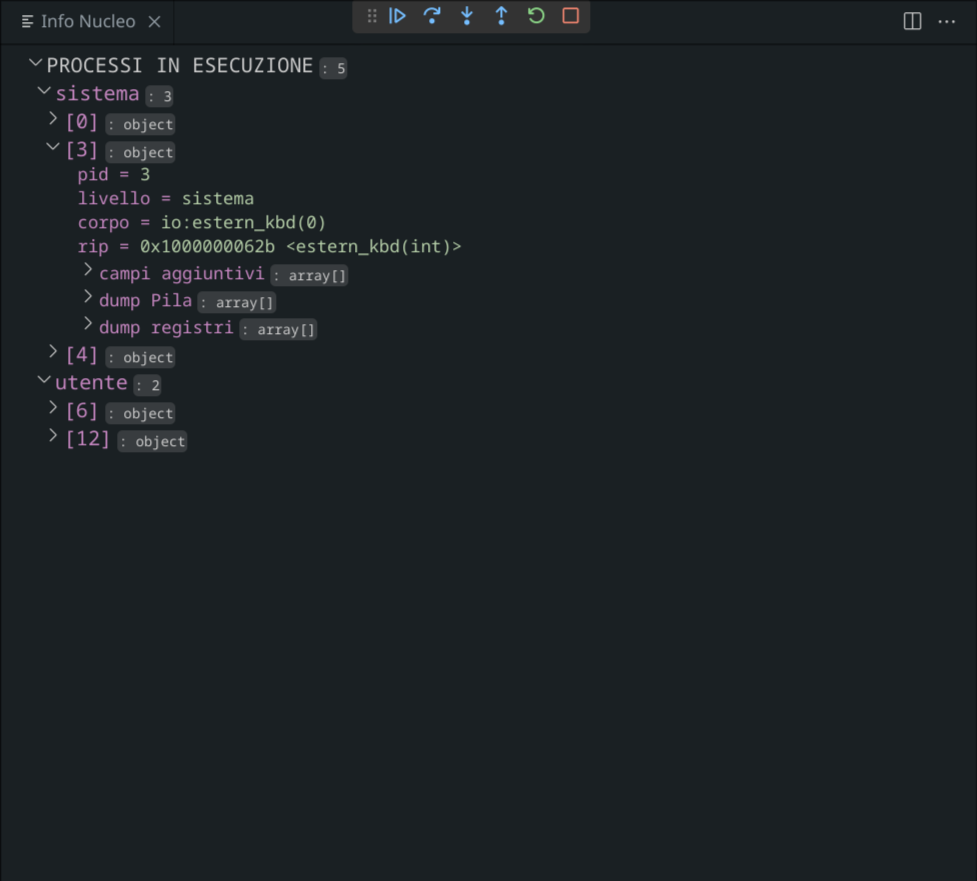
\includegraphics[width=0.7\columnwidth]{images/processes.png}
    \caption{Lista dei processi in esecuzione}
\end{figure}